\chapter{RooFit与GPU结合处理分辨率随能量变化的卷积问题研究}

物理实验中所有的探测器都会存在着一定的系统误差和统计误差,从而导致测量单能粒子得到的能谱不再是锐利的$\delta$函数,而会形成一定的展宽。展宽的大小可以用分辨率来描述,具体形状的数学描述公式通常被称为探测器的响应函数。探测器实际探测得到的能谱是粒子自身的本征谱与探测器响应函数的卷积。在一些如中微子能谱探测的实验中,粒子能谱跨度较宽、形式较为复杂\supercite{qian2015neutrino},需要考虑探测器能量分辨率随能量的变化的情况(经验上相对分辨率与待测能量呈下列关系:$\sigma_{E_0}=\sigma_0/\sqrt{E_0}$)\supercite{leo2012techniques},因此测量得到的能谱就不能表达成简单的卷积形式,也不能使用快速傅里叶变换来处理\supercite{mathworld},只能通过数值积分的方法求得函数的具体值。此时计算量会变的非常庞大,有些情况下,单纯使用CPU进行处理可能无法保障速度。这一章作者提出了一种使用GPU加速数值积分的方法,在保留原有RooFit (The Toolkit for Data Modeling with ROOT)\supercite{roofit}计算框架的基础上大大加快了计算速度,为形如中微子探测等相关实验中的数据处理提供相应的参考。

\section{积分原理部分分析}

为了能够快速地确认方法的可行性,我们使用了相对简单的柯西分布来代替探测前的粒子能谱,用高斯函数作为探测器的能量响应函数,这与X射线研究中的描述相类似\supercite{wang2006cmga}。首先,假设探测器能量分辨率不随能量变化而改变,此时卷积就可以通过既有的快速方法计算求得,从而可以检验该计算方法的可行性,然后再研究分辨率随能量变化时该方法的效率,以模拟真实情况。
柯西分布概率密度函数(Probability Density Function,PDF)为:
\begin{equation}
    f(x,x_0,\Gamma)=\frac{C}{(x-x_0)^2+(\frac{\Gamma}{2})^2}
\end{equation}

其中C为归一化系数,$x_0$和$\Gamma$为两待定参数。假设探测器的测量能量为t的粒子时,响应函数用均值为t,方差为$\sigma(t)$的高斯分布表示。那么探测器实际测量得到的中微子能谱即为两个函数的卷积,形式如下:
\begin{equation}
    g(x)=C'\int_{x_{min}}^{x_{max}}f(t,x_0,\Gamma)\cdot\frac{1}{\sigma(t)}\cdot e^{-\frac{(t-x)^2}{2\sigma^2(t)}}\cdot dt 
\end{equation}

其中$C'$为新的归一化因子,$x_{min}$和$x_{max}$是测量区域的下限和上限。如果$\sigma(t)\equiv\sigma_0$,此卷积结果即为Voigt函数,可以通过现有的快速算法计算得到\supercite{abrarov2011efficient}。因此我们将Voigt函数当作标准函数来检验积分的正确性。

常用的数值积分都可以写成被积函数f(x)的若干个函数值的线性组合,即:
\begin{equation}
    \int_a^bf(x)dx\approx\sum_{i=0}^n A_i f(x_i)
\end{equation}
其中Ai,xi与被积函数无关,称之为求积公式的系数和节点\supercite{jisuanfangfa}。通过合理的选择xi以及Ai就可以计算得到被积函数数值解。黎曼中点求积公式(以下称为黎曼积分)和高斯勒让德求积公式(以下称为高斯积分)是两种常见的数值积分方法\supercite{jisuanfangfa},适合于计算没有奇点的函数。其中黎曼积分的具体形式如下:
\begin{equation}
    \int_a^bf(x)dx = \sum_{i=0}^n \frac{1}{n}\cdot f(x_i)
\end{equation}
式中$x_i=a+\frac{b-a}{n}\cdot(i+\frac{1}{2})$。高斯积分形式如下:
\begin{equation}
\int_a^bf(x)dx=\frac{b-a}{2}\sum_{i=1}^n\omega_if(\frac{b-a}{2}x_i+\frac{b+a}{2})
\end{equation}
其中$x_i$是n阶勒让德多项式的零点,$\omega_i$为对应预先计算好的权重\supercite{jisuanfangfa}\supercite{bogaert2014iteration}。

从两种积分方式的公式可以看出,当积分范围确定后,两种积分方法所选择的节点和系数都与被积函数无关,这是一个良好的适合于并行计算的特性,同时可以通过缓存节点和系数来加速计算。

\section{RooFit介绍及使用CPU计算}

RooFit是CERN(欧洲核子研究组织)开发的基于C++的数据分析框架ROOT中重要组成部分\supercite{roofit}\supercite{root},它提供了许多高能物理数据分析中相关的工具,例如最大似然法无Bin拟合(unbinned maximum likelihood fits),Toy蒙特卡罗模拟,数据和函数的绘图等。RooFit提供了用于构造各类PDF的RooAbsPdf基类,在使用中只需要实现类中的evaluate()虚函数即可。而函数的归一化,以及使用该函数进行有bin拟合,无bin拟合等具体的实现则交由RooFit自动处理。因为RooFit的简化易用性,所以它在高能实验的数据分析软件中占了重要的地位。利用RooFit构造上述的概率密度函数只需要实现黎曼求积公式或者高斯求积公式的算法,并在evaluate()函数中调用对应算法计算函数值即可。其实现的伪代码如算法\ref{code:1}所示。

\begin{algorithm}  
    \caption{黎曼积分以及高斯勒让德积分}  
    \begin{algorithmic}[1] 
        \Require 
            $Xmax$,$Xmin$:积分上下界,$Bins$:分bin数目, $GaussLegendre$:高斯勒让德积分位置及权重信息
        \Ensure 
            积分结果
        \Function {RiemannEvaluate}{}
            \State $result \gets 0$  
            \State $step \gets (Xmax - Xmin) / Bins$
            \For{$i = 0 \to Bins$}
                \State $t \gets Xmin + (i + 0.5) * step$
                \State $result \gets result + $\Call{GetVal}{$t$}$ * step$
            \EndFor
            \State \Return{$result$}
        \EndFunction
        \Function{GausEvaluate}{}
            \State $result \gets 0$  
            \For{$i = 0 \to Bins$}
                \State $node \gets GaussLegendre[i]$
                \State $x \gets (Xmax-Xmin)/ 2 * node.x + (Xmax + Xmin) / 2$
                \State $result \gets result + node.weight * 
                $\Call{GetVal}{$x$}
            \EndFor
            \State $result \gets result * (Xmax – Xmin) / 2 $
            \State \Return{$result$}
        \EndFunction
    \end{algorithmic}  
    \label{code:1}
\end{algorithm}  

其中GetVal(t)函数返回被积函数在t处的值,Bins为节点数目。两种方法都是循环计算函数在各个节点上的值并依照权重求和。黎曼中点积分中节点均匀的分布在积分范围上,高斯勒让德积分则是使用预先计算好的节点位置和权重信息。在考虑到缓存节点位置和权重信息后,在取N个节点时两种积分方法的时间复杂度都是$O(N)$量级,计算整个PDF数值形式的时间复杂度为$O(N^2)$。在形如中微子能谱的数据处理过程中,中微子能谱本身形式复杂,能量跨度很大,因而需要较多的积分节点数目,使得计算速度大大降低。所以我们试图在两种积分算法中引入GPU运算,利用GPU众多的计算核心和并行能力来加速积分的运算,将GPU计算和RooFit框架结合起来,在享受框架带来便利的同时能够提高问题的解决速度。

\section{使用GPU加速积分过程}
随着计算需求的日益提高,传统模式下单纯的使用CPU进行串行计算已经不能满足人们的需求,于是多核心并行计算,网络分布式计算,FPGA编程等新型的计算模式逐渐走入了大众的视野。其中使用GPU进行加速计算无疑是最为火热的方法之一。在计算机发展历史中,GPU开始时只是专用于3D图像处理的硬件,正因为3D图像处理算法中有着大量的并行线性变换的需求,GPU从硬件设计上便考虑了并行算法的优化处理。2006年Nvidia公司为自家GPU推出了CUDA(Compute Unified Device Architecture,统一计算架构)技术\supercite{CUDA},而后2008年OpenCL(Open Computing Language,开放计算语言)也正式发布\supercite{opencl},GPU编程也正式的走出了图像处理领域,在通用计算中发挥了巨大的作用。

在硬件设计上GPU拥有着众多的计算单元和超长的流水线设计,但只有很简单的逻辑控制部分,因而相对于能够完成复杂逻辑运算的CPU,GPU更擅长于简单的重复性操作。在本文的卷积问题中,积分操作中函数值的计算就是这样一种简单重复的操作,只需将不同积分节点的计算任务分配给GPU的各个核心,然后再按照权重求和,就可以快速的得到最终的积分结果。

使用GPU进行黎曼积分的伪代码实现如算法\ref{code:2}所示。
\begin{algorithm}  
    \caption{使用GPU的黎曼积分}  
    \begin{algorithmic}[1] 
        \Require 
            $Xmax$,$Xmin$:积分上下界,$Bins$:分bin数目
        \Ensure 
            积分结果
        \Function {GPURiemannEvaluate}{}
            \State $result \gets 0$  
            \State $step \gets (Xmax - Xmin) / Bins$
            \State $t \gets $\Call{Sequence}{$Bins, Xmin + 0.5 * step, step$}
            \State $t \gets $\Call{Map}{$t$,GetVal}
            \State $result \gets step * $\Call{Reduce}{$t,0$,+}
            \State \Return{$result$}
        \EndFunction

    \end{algorithmic}  
    \label{code:2}
\end{algorithm} 
该伪代码中使用了三个函数式编程中的概念,即Sequence,Map,Reduce。 Sequence(count, start, step)类似于python中的range函数,用于生成一个起始值为start,间隔为step的长度为count的序列,并返回装有该序列的容器。Map (container, function)将function函数作用到容器中的每一个元素上,并将结果作为新的容器返回。Reduce (container, init, function)按照function函数合并容器里的所有元素,并返回最终结果。在该积分中,Sequence 产生了各个积分节点的位置,Map 给出了各个节点处函数的值,Reduce求和得到了最终的积分结果。

这三种操作中都是比较容易实现并行的,CUDA的开发环境中有一套名为thrust的并行计算库\supercite{thrust},它提供了GPU并行版本的Sequence, Map , Reduce方法 (即 thrust::sequence, thrust::transform, thrust::reduce),所以只需要编写能够在GPU上运行的GetVal核函数(kernel function)即可。

\section{测试与分析}

\subsection{正确性分析}

为了确定积分结果的正确性,即假设σ(t)≡σ0,此时积分结果应该与RooFit中Voigt函数(RooVoigtian)结果保持一致。取$\sigma \equiv 2.548, x_0=15, \Gamma=10,x_{max}=30,x_{min}=10$,此时探测器响应函数在x=20处的相对分辨率为30\%,Voigt函数的形式如图\ref{fig:cuda_com}中实线所示。

\begin{figure}
    \centering
    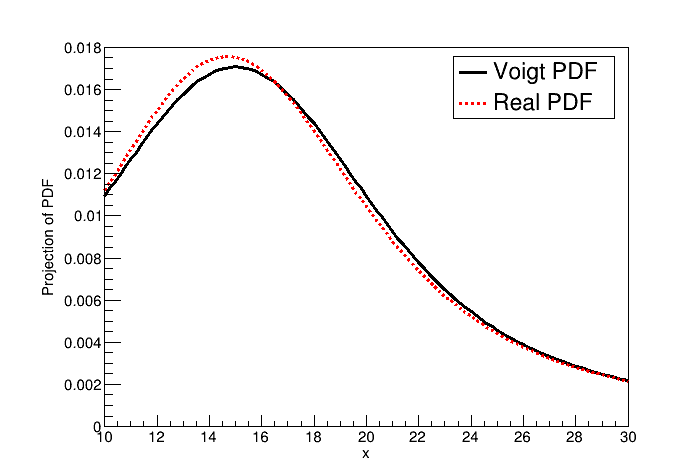
\includegraphics[width=0.6\columnwidth]{pic/cuda1.png}
    \caption{ Voigt概率密度函数(实线)以及考虑σ变化时实际概率密度函数(虚线)分布图。}
    \label{fig:cuda_com}
\end{figure}

为了验证积分的正确性,我们在x取值范围上均匀选取了10000个测试点,并用积分值与标准Voigt函数值的差的平方和来描述该积分的偏差。表\ref{tab:cuda_dif}给出了使用CPU进行黎曼积分,高斯积分以及使用GPU进行黎曼积分,高斯积分与Voigt函数的偏差,可以看出GPU给出了与CPU给出的结果完全完全一致,因为测试选用的被积函数十分的简单且变化平缓,本测试显示在节点数目达到100个后四种积分方式的偏差趋近于一个固定的小值,而这个值可以认为是Voigt函数使用傅里叶变换计算和数值积分计算两种算法之间的固定偏差。从总体来看四种数值积分方式得到的结果都是较为准确的。在实际的实验数据分析中,被研究粒子能谱自身形状可能会十分的复杂,例如在中微子实验中,理论上其能谱是一个复杂的含震荡的复杂形式,当节点数目较小时数值积分可能会带来较大的偏差。因此在效率允许的情况下数值积分的节点应足够多以满足精度要求。

\begin{table*}
    \centering
    \begin{tabular*}{\textwidth}{@{\extracolsep{\fill}}cccc}
        \hline
        \hline							
        方法	&	10节点时偏差	&	100节点时偏差	&	1000节点时偏差	\\\hline
        黎曼积分	&	$1.63124\times10^{-2}$	&	$9.10558\times10^{-2}$	&	$9.20354\times10^{-2}$	\\
        高斯积分	&	$2.57649\times10^{-1}$	&	$9.20453\times10^{-2}$	&	$9.20453\times10^{-2}$	\\
        使用GPU的黎曼积分	&	$1.63124\times10^{-2}$	&	$9.10558\times10^{-2}$	&	$9.20354\times10^{-2}$	\\
        使用GPU的高斯积分	&	$2.57649\times10^{-1}$	&	$9.20453\times10^{-2}$	&	$9.20453\times10^{-2}$	\\
        \hline
        \hline
    \end{tabular*}
    \caption{不同节点数目时候四中积分结果相较于Voigt函数的偏差。}
    \label{tab:cuda_dif}
\end{table*}

\subsection{性能分析}

随后我们测试了四种积分方法在考虑$\sigma$变化情况(Real PDF)下的性能。被积函数中$\sigma(t)=2.458\times\sqrt{t/20}, x_0=10, \Gamma=10,x_{max}=30,x_{min}=10$,如图\ref{fig:cuda_com}中红色虚线所示。可以看出$\sigma$随能量变化的情况会最终影响PDF分布。如上节一样,本文统计四种方法在10000个测试点处的平均耗时,以此来比较它们的性能。统计得到的时间消耗随节点数目变化如图\ref{cuda_2}所示。因为在节点数目较高时使用CPU方法所消耗的时间过长,所以图中使用CPU的方法最大只测试了$1\times10^6$个节点。

\begin{figure}
    \centering
    \includegraphics[width=0.6\columnwidth]{pic/c1.pdf}
    \caption{ 基于CPU的黎曼积分(CPU Riemann),高斯积分(CPU Gauss),GPU加速的黎曼积分(GPU Riemann)以及GPU加速的高斯积分(GPU Gauss)四种积分方法的时间消耗与节点数目的关系。}
    \label{fig:cuda_2}
\end{figure}

从图中可以看出CPU计算代码的时间消耗随bin数目增加而线性的增长,高斯积分的效率略低于黎曼积分。这是因为高斯积分的权重值是不一致的,虽然可以缓存权重值,但是与黎曼积分中常数权重相比还是会慢一些。在测试机器上,GPU的两种算法在节点数目小于$2\times10^5$的时候时间消耗基本不变,在节点数目大于$1\times10^6$后时间消耗也随节点数目线性增长。理想情况下如果GPU核心数目足够多,那么上述伪代码中的Sequence,Map 操作的时间复杂度为$O(1)$,而Reduce 操作的可以通过两两合并实现,时间复杂度为$O(\log{n})$。但是因为GPU运算需要进行初始化等操作,所以当节点数目较少计算量较小时,GPU不能满载运行,计算时间消耗到了固定初始化操作。而当节点数目较多计算量过大时,GPU核心数目也达到了阈值,因而时间消耗随节点数目线性增长。通过计算CPU积分和GPU积分两种算法所耗时间的比值,就可以得到使用GPU所带来的性能提升,如表\ref{tab:cuda_2}所示:在被积函数非常复杂需要很多节点以达到精度时,GPU能够提高计算性能,在节点数目较小时CPU反而能够更快的达到计算目标。当节点数目为$1\times10^6$时,使用GPU进行高斯积分,黎曼积分时能够将速度提高168倍以及203倍。

\begin{table*}
    \centering
    \begin{tabular*}{0.8\textwidth}{@{\extracolsep{\fill}}cccc}
        \hline
        \hline							
        节点数目	&	高斯积分	&	黎曼积分	&	优化后黎曼积分	\\\hline
        $1\times10^3$	&	0.23	&	0.35	&	0.79	\\
        $2\times10^3$	&	0.46	&	0.65	&	1.56	\\
        $5\times10^3$	&	1.14	&	1.66	&	3.9	\\
        $1\times10^4$	&	2.28	&	3.31	&	7.8	\\
        $2\times10^4$	&	4.48	&	6.58	&	14.9	\\
        $5\times10^4$	&	11.3	&	16.4	&	37.8	\\
        $1\times10^5$	&	22.5	&	32.1	&	73.5	\\
        $2\times10^5$	&	44	&	63.2	&	105	\\
        $5\times10^5$	&	110	&	156	&	186	\\
        $1\times10^6$	&	168	&	203	&	218	\\
        \hline
        \hline
    \end{tabular*}
    \caption{相对于CPU而言,使用GPU进行高斯积分、黎曼积分以及优化后的黎曼积分所带来的性能提升。}
    \label{tab:cuda_2}
\end{table*}


\subsection{性能优化}

从上节中可以看出在较少节点数目的时候GPU计算性能相对较低,经过对代码分析后发现时间主要消耗到了thrust的reduce函数。进一步研究thrust库中相关代码可以发现,它的实现并不是最优化的两两合并,而是采用了分治的思想,将reduce容器分成若干块,每一块都由一个GPU计算核心顺序的进行reduce操作,将结果储存在一个临时的容器中,随后再使用一个核心来reduce这个临时容器。这种实现可以避免多次初始化GPU计算核心,降低操作的延迟。但是thrust为了通用性考虑,每次reduce操作时所需要的临时容器都会重新建立,这一GPU显存操作会带来极大地时间消耗。而在卷积操作时,节点数目一般是预先设定好的,故reduce操作所需要的临时容器的大小也是可以确定的,因而预先申请该空间并重复利用来提升reduce操作的性能。优化过reduce操作的黎曼积分和未优化的性能对比如图\ref{fig:cuda_3}所示。

从图\ref{fig:cuda_2}和图\ref{fig:cuda_3}中也可以看出在节点数目低于一定阈值$(C0)$的时候,GPU积分计算所消耗的时间基本上是一个常数,正如上节性能分析中所说,此时GPU并没达到满载工作,核心数目满足积分计算的需求,大部分计算时间消耗到了初始化等操作中。即增加GPU的核心数目只能够提高节点数目的阈值$(C0)$的大小。所以当被积分函数形式复杂,变化剧烈,需要超过阈值$(C0)$个积分节点来保障描述函数变化细节时,增加GPU核心数目能够提高计算的性能。 

\begin{figure}
    \centering
    \includegraphics[width=0.6\columnwidth]{pic/c2.pdf}
    \caption{ 使用CPU的黎曼积分(CPU Riemann),使用GPU的黎曼积分(GPU Riemann)以及优化后的黎曼积分(GPU Riemann Tuned)积分耗时与节点数目的关系。}
    \label{fig:cuda_3}
\end{figure}

\section{小结}

在例如中微子的能谱等相关的研究中,因为能谱涉及范围大,能谱复杂,在数据拟合分析时需要考虑到探测器分辨率随能量变化的情况。本文研究了使用GPU配合RooFit来处理能谱卷积问题,给出了相关的示例代码并验证了算法的正确性。从时间消耗上来看GPU更擅长于处理复杂函数,当问题比较复杂,计算量较大时使用GPU能够显著地提高计算性能,节约数百倍的时间,而当所需积分节点数目较小时性能往往不如CPU。此章节给出的GPU数值积分方法也适用其它各种含积分形式的概率密度函数的计算中,可为类似实验数据分析算法提供参考。